\documentclass[11pt,letterpaper]{article}
\usepackage[utf8]{inputenc}

%----- Configuración del estilo del documento------%
\usepackage{epsfig,graphicx}
\usepackage[left=2cm,right=2cm,top=1.8cm,bottom=2.3cm]{geometry}
\usepackage{fancyhdr}
\usepackage{lastpage}

\usepackage{xcolor}
\usepackage{soul}
\newcommand{\mathcolorbox}[2]{\colorbox{#1}{$\displaystyle #2$}}

%Color bibi
\definecolor{bibi}{RGB}{0,103,148}
% Otros colores

%------ Paquetes matemáticos básicos --------%
\usepackage{amsmath}
\usepackage{amssymb}
\usepackage{amsthm}

%------ Paquetes para codigo --------%
\usepackage{verbatim}
\usepackage{listings}
\lstset{language=Haskell, basicstyle=\ttfamily, keywordstyle=\color{blue}, commentstyle=\color{gray}, stringstyle=\color{green}}

\usepackage{tikz}


\begin{document}

%------ Encabezado -------- %
\begin{center}
    \begin{minipage}{3cm}
    	\begin{center}
    		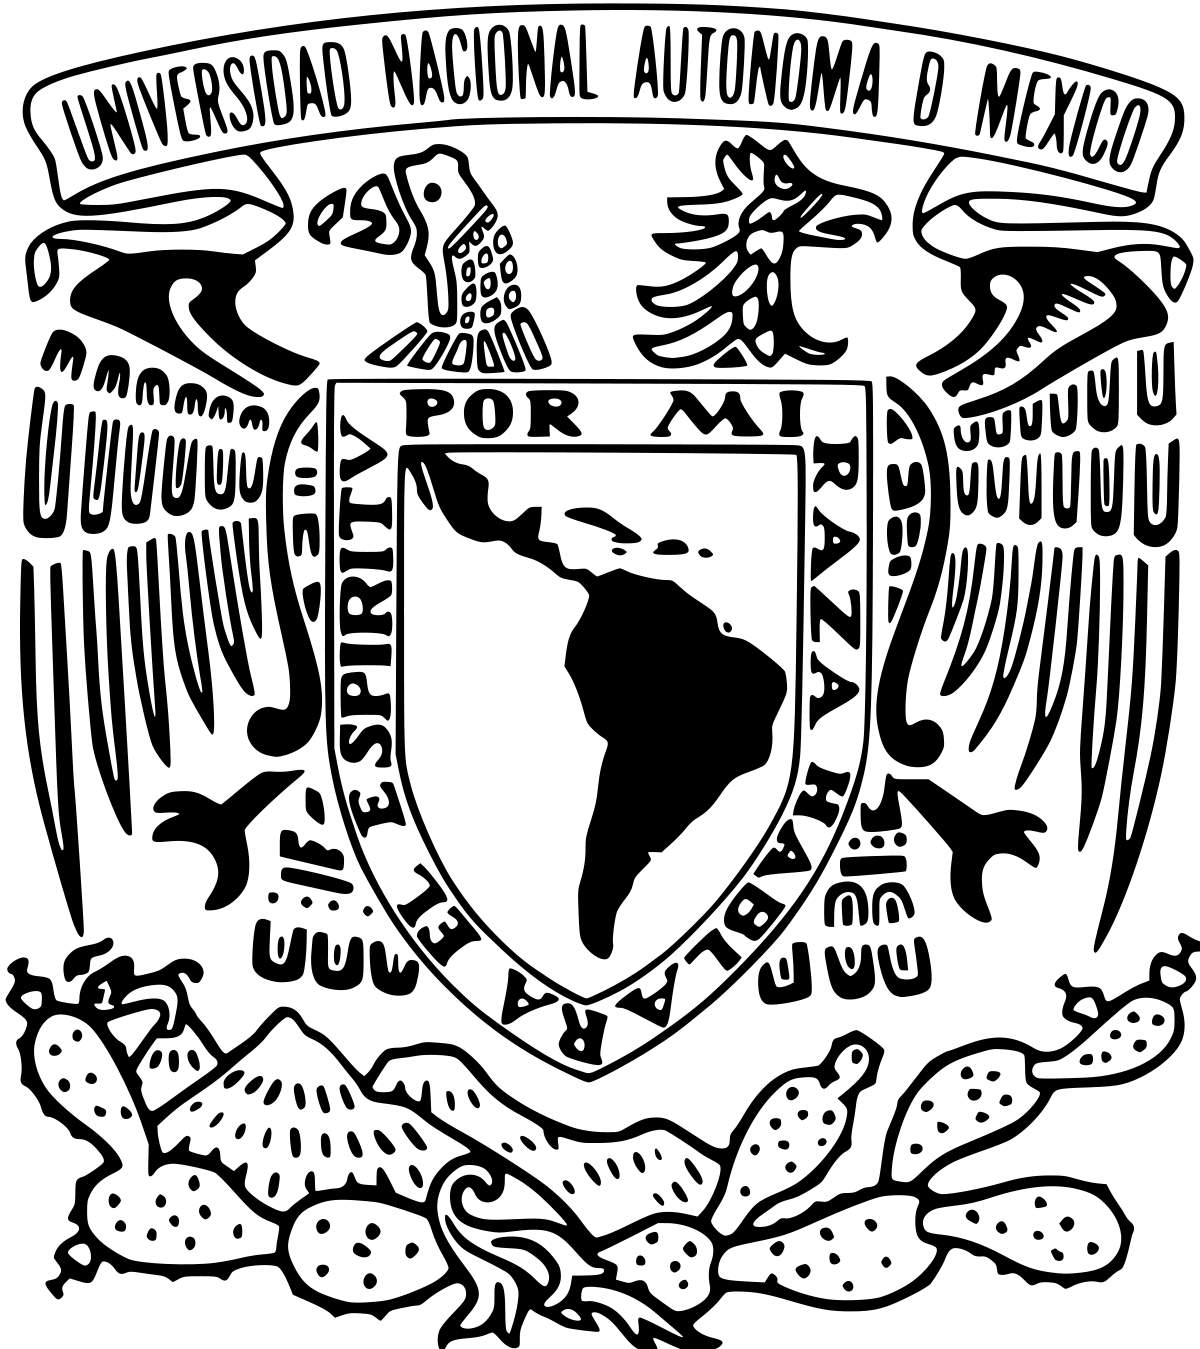
\includegraphics[height=3.2cm]{src/Img/Logo_UNAM.png}
    	\end{center}
    \end{minipage}\hfill
    \begin{minipage}{10cm}
    	\begin{center}
    	\textbf{\large Universidad Nacional Autónoma de México}\\[0.1cm]
        \textbf{Facultad de Ciencias}\\[0.1cm]
        \textbf{Taller intersemestral Communitario}\\[0.1cm]
        Tarea 1: $|$ Diseño de proyecto \\[0.1cm]
        Sosa Romo Juan Mario $|$ 320051926 \\[0.1cm]
        30/06/25
    	\end{center}
    \end{minipage}\hfill
    \begin{minipage}{3cm}
    	\begin{center}
    		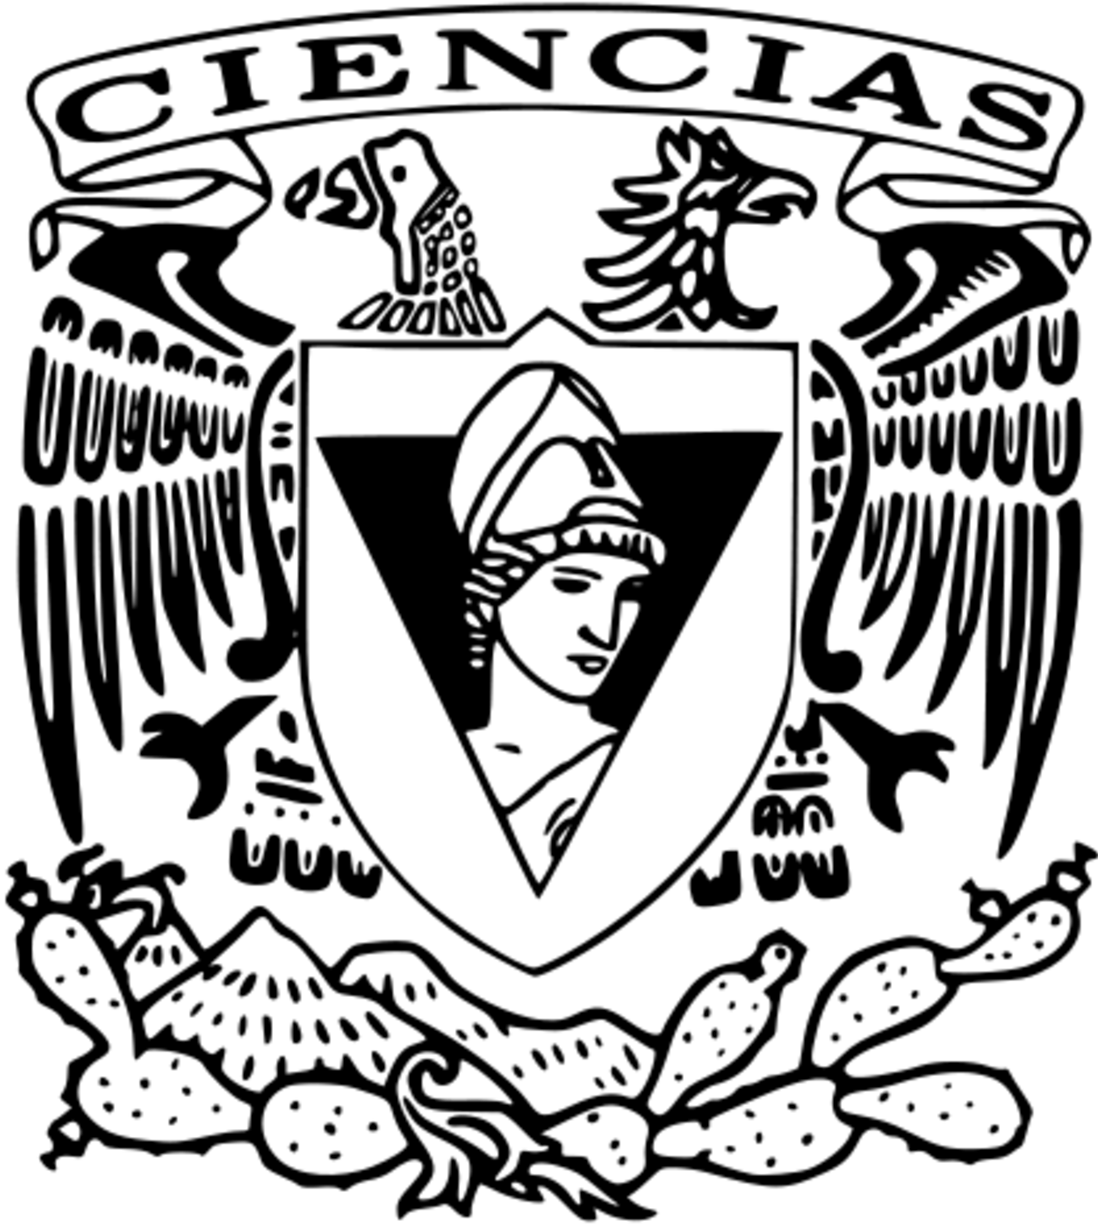
\includegraphics[height=3.2cm]{src/Img/Logo_FC.png}
    	\end{center}
    \end{minipage}
\end{center}


\rule{16.9cm}{0.1mm}
\vspace{0.3cm}

\vspace{0.3cm}
%------ Preguntas -------- %
\begin{enumerate}
    \item \textbf{Objetivo del proyecto + metodo smart}\vspace{.5cm}


Antes de redactar en el formato \texttt{SMART} el que del proyecto; voy a explicar a grandes razgos que espero conseguir. \vspace{.3cm}

La idea es poder tener un comando en terminal ya sea usando bash o python, que sea capaz de recibir un chat exportado de whatsap y darme estadisticas relevantes del mismo. Algunas ideas principales podrian ser: 

\begin{itemize}
    \item Conseguir las frases mas recurrentes
    \item Conseguir las palabras mas recurrentes
    \item Ver la cantidad de mensajes por individuo (todavia no se si va a funcionar tambien para chats grupales)
    \item Ver los horarios mas frecuentes 
    \item Longitud promedio de mensajes 
    \item Datos de imagenes/ emojis (todavia no estoy seguro de eso)
    \item Otras metricas que vaya encontrando en el camino
\end{itemize}

Lo anterior cubre, el ser especifico y medible, ademas de ser alcanzable y creo se puede realizar en el tiempo especificado de la entrega.   \vspace{.3cm}

Finalmente, para la relevancia, surgio de un argumento que tuve con un amigo sobre quien preguntaba mas un tipo de pregunta especifica, en el momento cree un scrip de python con gpt y use colab para correr y encontrar este caso especifico, pero creo que podria extenderlo mas y abstraerlo (ademas de mejorarlo). \vspace{.3cm}
\end{enumerate}

\end{document}